\documentclass[11pt,a4paper]{article}
\usepackage[T1]{fontenc}
\usepackage[utf8]{inputenc}
\usepackage{lmodern}
\usepackage[margin=25mm]{geometry}
\usepackage{amsmath,amssymb}
\usepackage{graphicx}
\usepackage{booktabs}
\usepackage{microtype}
\usepackage[numbers,sort&compress,square]{natbib}
\usepackage[colorlinks=true,citecolor=blue,linkcolor=blue,urlcolor=blue]{hyperref}
\usepackage{caption}
\usepackage{placeins}
\captionsetup{font=small,labelfont=bf}
\setlength{\emergencystretch}{2em}
\newcommand{\forceunit}{\ensuremath{\mathrm{eV}\,\text{\AA}^{-1}}}
\newcommand{\coreh}{\ensuremath{\mathrm{core\!-\!h}}}
% Author-supplied metadata. These explicit placeholders must be replaced before submission.
\newcommand{\PaperAuthors}{[Author names to be supplied]}
\newcommand{\PaperAffiliations}{[Affiliations to be supplied]}
\newcommand{\PaperContact}{[Corresponding-author email to be supplied]}
\newcommand{\PaperAcknowledgments}{[Funding and acknowledgments to be supplied by the authors.]}

\title{PHAL: Physics-Aware Hotspot Active Learning\\
for Local Reference Labeling of Machine-Learned Force Fields}
\author{\PaperAuthors\\[0.4em]\small \PaperAffiliations\\\small \PaperContact}
\date{}

\begin{document}
\maketitle
\begin{abstract}
Local reference calculations can reduce the cost of extending a machine-learned
force field, but their use requires control of fragment-boundary errors and a
reliable path from molecular dynamics to model updates. We present the
Physics-aware Hotspot Active Learning Platform (PHAL), implemented in
GMD\_active and connected to the GMD dynamics engine, CP2K reference calculations,
and GMD\_SGT training. The workflow combines staged heuristic monitoring,
event-based hotspot selection, hydrogen-capped extraction, weighted force
supervision, and persistent execution with model-promotion checks.
Completed exploratory experiments use hexadecane and dotriacontane configurations
with torsional, bending, and nonbonded-contact perturbations. A fragment setting
selected on hexadecane reproduces held-out parent core forces with a
Cartesian-component root-mean-square error of 0.0100~\forceunit; unchanged
transfer to two dotriacontane configurations gives 0.0146~\forceunit.
An exploratory four-label comparison gives mean force errors of
0.479 and 0.502~\forceunit\ for local and full-system PHAL labeling, with
an attributed reference-cost ratio of 0.19; two repetitions and incompletely
paired acquisitions preclude an equivalence claim.
A separate real-program closed loop adds three local labels and reduces
validation error from 0.506 to 0.398~\forceunit. In short frozen-model
trajectories, the fraction of sampled frames retaining the parent bond topology
increases from 36.6\% to 98.7\%.
These results establish an operational framework and pilot-scale label fidelity,
while leaving acquisition superiority, the incremental value of physical
signals, and repair of an initially qualified force field unresolved.
\end{abstract}

\noindent\textbf{Keywords:} active learning; machine-learned interatomic potentials;
local reference labeling; molecular dynamics; fragment fidelity; reproducibility

\section{Introduction}
Machine-learned interatomic potentials approximate a reference potential-energy
surface at a cost that permits molecular-dynamics (MD) sampling beyond typical
first-principles trajectories. Their usefulness depends on the environments
represented by the training data. A model can perform adequately on familiar
structures yet make consequential force errors when a trajectory reaches
an unfamiliar local arrangement. Active learning addresses this problem
by deciding where reference calculations should be added and incorporating
the resulting data into subsequent models. D-optimality-based selection
for moment tensor potentials and Bayesian on-the-fly force fields provide
established examples of this strategy
\citep{podryabinkin2017active,vandermause2020flare}.

An operational active-learning system also has to connect exploration,
reference labeling, and training. DP-GEN implements this cycle through
modular simulation and labeling backends \citep{zhang2020dpgen}.
For a large parent structure, however, even a single whole-system reference
calculation may be expensive. Local selection offers an additional way to
control this cost. Hodapp and Shapeev identify extrapolative subregions and
construct small periodic reference systems \citep{hodapp2020inoperando};
MLIP-3 supports active learning on atomic neighborhoods
\citep{podryabinkin2023mlip3}. Thus neither the closed loop nor the principle
of local active learning is introduced here.

Covalently connected molecules make the validity of local labels particularly
important. Cutting out a neighborhood changes its electronic environment and
can create unsaturated bonds. Hydrogen termination restores a closed-shell
fragment for the alkane systems considered here, but it does not guarantee
that all fragment forces equal their parent counterparts. Boundary atoms and
artificial caps can therefore require different treatment from the region
whose force is intended to be learned. A second, distinct issue is that the
learned model itself may depend on an environment larger than the retained
fragment. Reliable use of local supervision requires these two questions to
be kept separate.

This work presents the Physics-aware Hotspot Active Learning Platform
(PHAL) as implemented in GMD\_active. PHAL connects the GMD MD engine,
CP2K density-functional theory (DFT) calculations, and the GMD\_SGT
potential-training backend. The central implementation choices are staged
heuristic monitoring, event-based localization, explicit fragment-fidelity
checks, role-dependent force weights, and persistent workflow state.
GMD and GMD\_SGT denote the dynamics and training components of the
ecosystem; GMD\_active owns the active-learning logic.

We evaluate three questions using completed alkane pilot experiments:
whether capped fragments reproduce parent core forces within stated
tolerances; whether the software executes acquisition, labeling, and training
with traceable costs; and whether a real closed loop changes model error
and short-trajectory behavior. We retain unsuccessful configurations and
unexercised acquisition cases. The results support the feasibility of local
supervision and the operation of the implementation. They do not establish
that PHAL is a generally better acquisition policy or that its physical
features provide calibrated uncertainty.

\begin{figure}[tb]
  \centering
  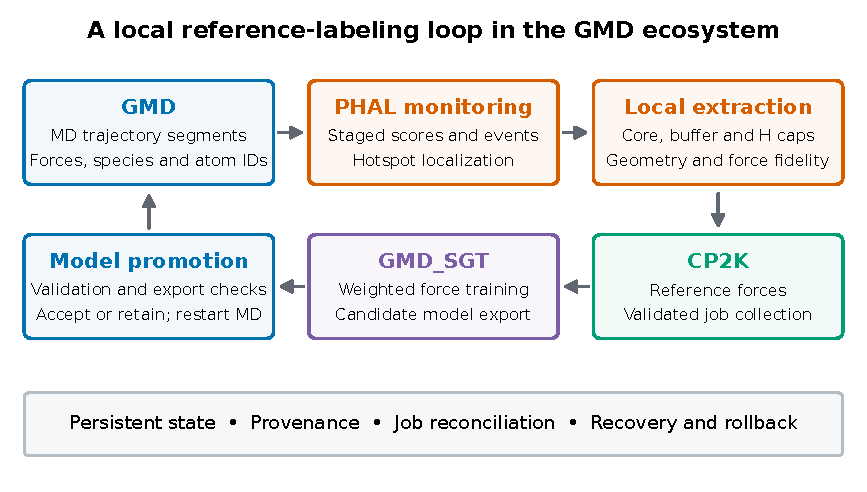
\includegraphics[width=\linewidth]{figures/fig01_workflow.pdf}
  \caption{PHAL within the GMD ecosystem. GMD produces trajectory segments;
  GMD\_active performs monitoring, extraction, job orchestration, and model
  promotion; CP2K provides reference labels; and GMD\_SGT trains and exports
  candidate models. Persistent records connect events, labels, datasets, and
  model versions. The diagram describes software responsibilities, not a
  guarantee that every candidate will be labeled or every trained model
  promoted.}
  \label{fig:workflow}
\end{figure}

\section{Methods and implementation}
\subsection{Interfaces and persistent execution}
Figure~\ref{fig:workflow} summarizes the separation of responsibilities.
The MD interface supplies positions, forces, species, stable atom identities,
cell information, and step indices. Segmented execution provides explicit
restart boundaries at which an accepted model can replace the active model.
Simulation state and model identity are recorded together so that a resumed
segment can be traced to the potential that generated it.

The controller persists its stage and records intended external actions,
their execution, and their outcomes. On restart, unresolved actions are
reconciled against the relevant backend before a new job is submitted.
Event, label, dataset, and model identities link the corresponding records.
The SQLite store uses write-ahead logging and uniqueness constraints.
These mechanisms support the recovery experiments reported below; their
presence alone is not evidence of correctness under every scheduler or
distributed failure mode.

Reference calculations are collected and validated before they enter a
dataset. Model promotion is separate from model training: a candidate must
pass the configured validation, export-consistency, and engine checks.
A rejected candidate leaves the accepted model available. The pilot uses
permissive promotion thresholds, stated in Section~\ref{sec:protocol};
passing those checks is not interpreted as proof of an accurate force field.

\subsection{Monitoring, events, and hotspot selection}
The monitoring interface supports force magnitude, force change,
nearest-neighbor distance, displacement, coordination change, local
Lennard--Jones (LJ) compatibility, and committee force dispersion.
Metrics are scheduled in a light stage, a physics stage, and a full stage.
For atom $i$ and stage $s$, the configured aggregate has the form
\begin{equation}
 S_i^{(s)}=\sum_{k\in\mathcal{K}_s}w_k g_k(x_{ik}),
 \label{eq:score}
\end{equation}
where $g_k$ is a metric-specific transformation and $w_k$ is a configured
weight. Several transformations use gated absolute standardized deviations
from running statistics. Other metrics retain raw-value contributions.
Unavailable metrics contribute zero and are excluded from the associated
statistics. Consequently, these aggregates are heuristic trigger scores,
not calibrated probabilities of reference-force error.

The pilot stage thresholds are 4, 5, and 6, with one atom sufficient to
trigger a stage. Under triggered scheduling, a lower-stage decision
controls whether the next stage is evaluated. The implementation can instead
evaluate stages unconditionally; the exploratory static-pool experiment
uses this option. The executed online pilot disables force-change,
displacement, coordination-change, and separate reference-model-deviation
metrics. It therefore does not validate every temporal feature available
in the platform.

For a committee of $M$ models, the force-dispersion feature is
\begin{equation}
 u_i=\left[\frac{1}{M}\sum_{m=1}^{M}
 \left\|\mathbf{F}^{(m)}_i-\overline{\mathbf{F}}_i\right\|^2\right]^{1/2},
 \qquad
 \overline{\mathbf{F}}_i=\frac{1}{M}\sum_{m=1}^{M}\mathbf{F}^{(m)}_i .
 \label{eq:committee}
\end{equation}
It is a population dispersion of force vectors, without an additional
factor of three.

The LJ feature fits the current predicted force to two local geometric
basis vectors. With $\mathbf{d}_{ij}=\mathbf{r}_j-\mathbf{r}_i$ and
$r_{ij}=\|\mathbf{d}_{ij}\|$,
\begin{align}
 \mathbf{a}_i&=-2\sum_j\frac{\mathbf{d}_{ij}}{r_{ij}^{14}},
 & \mathbf{b}_i&=\sum_j\frac{\mathbf{d}_{ij}}{r_{ij}^{8}},\\
 \widehat{\mathbf{F}}^{\rm LJ}_i&=\alpha_i\mathbf{a}_i+\beta_i\mathbf{b}_i,
 & \rho_i&=\frac{\|\widehat{\mathbf{F}}^{\rm LJ}_i-\mathbf{F}_i\|}
 {\|\mathbf{F}_i\|+\delta}.
 \label{eq:lj}
\end{align}
Here $\alpha=24\epsilon\sigma^{12}$ and
$\beta=24\epsilon\sigma^6$ for the conventional LJ potential, and the force
sign follows $\mathbf{F}=-\nabla E$. The pilot fits each atom separately
using neighbors within 6~\AA, including covalently bonded neighbors.
Rank, conditioning, positivity, and length-scale checks reject unsuitable
fits (Appendix~\ref{app:settings}). This is a compatibility feature for a
simple pair-force form. It is not a physicality certificate for a covalent
force field. Two fitted coefficients span a plane in three-dimensional
force space, and a positive uniform force rescaling can be absorbed into
the fitted energy scale.

Triggered frames are retained with configured pre- and post-trigger
context. Additional triggers within a pending event merge reasons,
scores, and hotspot identities; incomplete events are marked explicitly.
Trigger-frame identities are retained separately from later event members.
Hotspot atoms are clustered by a 3~\AA\ single-linkage distance.
Candidates are ranked by score, then filtered against selected and
previously labeled geometric fingerprints. The pilot uses a fingerprint
distance threshold of 0.1. These filters can determine the acquired
labels even when many frames trigger.

\subsection{Extraction, capping, and a fragment-fidelity gate}
The implementation offers graph, radial-cluster, block, and slab extraction.
The molecular experiments here assess graph and radial extraction only.
Whole carbon--hydrogen units are retained so that terminal hydrogens
follow their bonded carbon. Every severed carbon--carbon bond is
terminated by a hydrogen at 1.09~\AA\ along the cut-bond direction.
Caps are not relaxed in these experiments.

The calibration compares graph neighborhoods of two, three, and four
carbon--carbon bond hops with radial neighborhoods having a
1.5~\AA\ core and buffers of 3, 4, or 5~\AA.
For a perturbation site consisting of several atoms, the radial
neighborhood is the union of their neighborhoods; it is not necessarily
a sphere about a single atom. Parent identities, retained-atom identities,
region roles, and cap records are preserved.

Each candidate extraction setting is checked against parent DFT forces
computed with the same electronic-structure settings. Over the evaluated
core atoms $\mathcal{C}$, the gate measures the component root-mean-square
error (RMSE) and maximum atomwise vector error:
\begin{align}
 R_{\rm core}&=
 \left[\frac{1}{3|\mathcal{C}|}
 \sum_{i\in\mathcal{C}}\|\mathbf{F}^{\rm frag}_i-
                         \mathbf{F}^{\rm parent}_i\|^2\right]^{1/2},\\
 E_{\max}&=\max_{i\in\mathcal{C}}
 \|\mathbf{F}^{\rm frag}_i-\mathbf{F}^{\rm parent}_i\|.
 \label{eq:fidelity}
\end{align}
Acceptance requires $R_{\rm core}\leq0.03$~\forceunit,
$E_{\max}\leq0.10$~\forceunit, complete evaluation, and no failed
fragment. The lowest measured mean-cost passing setting is selected;
a fixed order resolves a cost tie. The settings and acceptance criteria
were recorded before the fidelity sweep. This local protocol record
is not an external preregistration.

\subsection{Force supervision and model updates}
Local datasets distinguish core, inner-buffer, outer-buffer, boundary,
and cap atoms. In the executed study, force weights are 1 for the core,
0.3 for the inner buffer, and zero for the outer buffer, boundary,
caps, and unassigned atoms. Full-system force labels have unit weights.
The weighted force root-mean-square loss is
\begin{equation}
 L_F=\left[
 \frac{\sum_i w_i\sum_{\mu\in\{x,y,z\}}
 (F_{i\mu}^{\theta}-F_{i\mu}^{\rm ref})^2}
 {3\sum_i w_i}\right]^{1/2}.
 \label{eq:loss}
\end{equation}
The implementation handles a zero-weight batch explicitly and uses a
numerical floor for a finite derivative at zero error. Zero-weight targets
contribute neither a force-loss term nor a force gradient.
Capped-fragment energies are excluded from energy supervision: a fragment
energy is not a parent energy or an additive parent-energy contribution.
Full-system labels retain their own energy targets.

Local DFT fidelity and learned-model context are separate constraints.
Equation~\eqref{eq:fidelity} tests whether the reference forces survive
fragmentation. It does not test whether the trained model predicts the
same core force on the fragment and its parent. We report the completed
model-context diagnostic as a limitation rather than treating a DFT gate
pass as evidence that the learned representation is insensitive to
removed neighbors.

\section{Experimental setup}
\label{sec:protocol}
\subsection{Molecular configurations and data splits}
The C16 pilot comprises 16 neutral, closed-shell
$\mathrm{C}_{16}\mathrm{H}_{34}$ parents: four base conformations,
each with an ordinary, torsional, bent, and contact configuration.
A base is an ideal all-trans chain together with a seeded Gaussian
displacement field of standard deviation 0.03~\AA\ per Cartesian
component. The same field is applied after each perturbation derived
from that base. Carbon--carbon and carbon--hydrogen bond lengths before
perturbation are 1.53 and 1.09~\AA, respectively, with tetrahedral angles.
The Atomic Simulation Environment (ASE) supports atomistic structure handling
\citep{larsen2017ase}.

Torsion rotates one connected side of a carbon--carbon bond; bending
rotates one connected side about a backbone vertex. Nonbonded contacts
are generated by folding consecutive torsions subject to topology and
clash constraints. Geometry checks reject changed bond topology,
inconsistent rigid operations, unacceptable bonds or angles, and
nonbonded clashes. Figure~\ref{fig:structures} shows the four actual
held-out C16 structures used in the pilot.

One base is assigned to each of the initial-training, calibration,
validation, and final-evaluation partitions, giving four structures per
partition. All structures derived from a base remain together.
This separation avoids direct sharing of a base displacement field
between partitions, but all four bases are closely related perturbations
of an all-trans chain; they are not a broad sample of equilibrium
conformations. A size-transfer check uses two
$\mathrm{C}_{32}\mathrm{H}_{66}$ parents from a single base, one torsional
and one contact configuration. It retains the extraction setting chosen
on C16 without reselection.

\begin{figure}[tb]
  \centering
  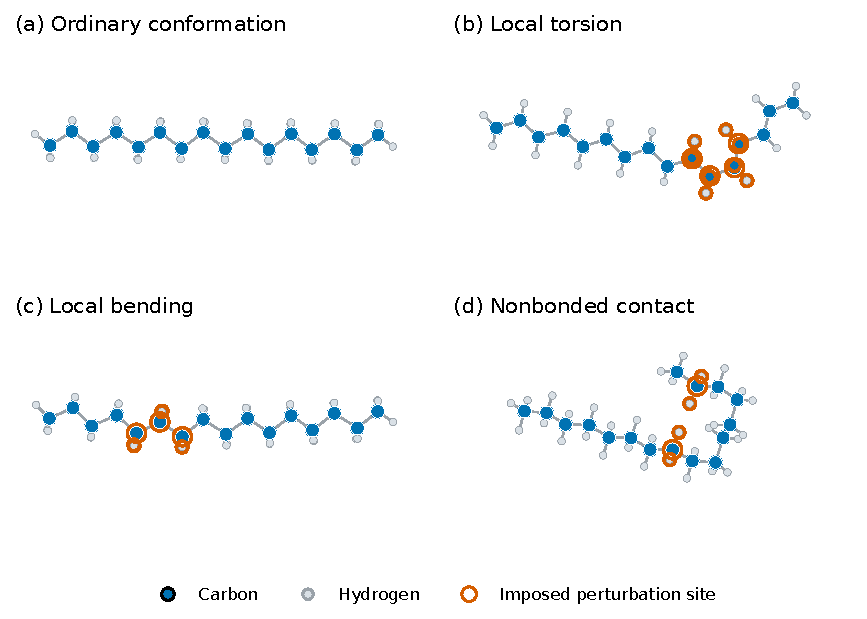
\includegraphics[width=\linewidth]{figures/fig02_configurations.pdf}
  \caption{Actual C16 final-evaluation structures: ordinary, torsional,
  bent, and folded-contact configurations. Carbon atoms are blue and
  hydrogen atoms light gray. Orange outlines indicate the imposed
  perturbation-site atoms from the generation record, not model-detected
  hotspots. Each structure is projected onto its own first two principal
  axes using the same spatial scale. These illustrations are generated
  from stored coordinates, not from a molecular image generator.}
  \label{fig:structures}
\end{figure}

\subsection{Reference calculations}
CP2K \citep{kuhne2020cp2k} supplies parent and fragment references using
the Perdew--Burke--Ernzerhof functional \citep{perdew1996pbe} with
DFT-D3 dispersion and Becke--Johnson damping
\citep{grimme2010d3,grimme2011d3bj}.
The basis is DZVP-MOLOPT-SR-GTH with GTH-PBE pseudopotentials;
the molecularly optimized basis construction is described in
Ref.~\citep{vandevondele2007molopt}.
Calculations use a singlet restricted description, 300~Ry cutoff,
50~Ry relative cutoff, and a self-consistent-field (SCF) tolerance
of $10^{-6}$. The initial solver uses orbital transformation with
a 100-iteration limit and a bounded retry policy.
Parents and fragments have identical electronic-structure settings.
An isolated WAVELET Poisson solver uses a cubic box enclosing the
structure with 6~\AA\ padding on each side.
The recorded cutoff probe gives a root-mean-square force difference of
approximately 0.006~\forceunit\ between 300/50 and 400/60~Ry; this is a limited
numerical probe, not a general convergence guarantee.

All reported reference jobs use one process with five OpenMP threads.
Cost is measured wall time multiplied by allocated cores and summed
over attempts, including failures and retries. This quantity is an
allocation measure, not a direct hardware-counter measurement of CPU
utilization. A reused label incurs no new computation, but an
acquisition arm is charged that label's historical measured cost
when comparing reference-data requirements.

\subsection{Potential and acquisition experiments}
GMD\_SGT trains a local equivariant potential with two blocks, scalar
dimension 32, representations $32\times0e+8\times1o$, eight radial
basis functions, and a 4~\AA\ local cutoff. No long-range term is enabled.
A primary model and two additional members form the committee.
The exploratory static-pool study uses at most 1500 training epochs,
batch size one, initial learning rate $2\times10^{-3}$, and patience
300. Energy-per-atom mean-absolute error and force RMSE have coefficients
0.1 and 1, respectively.

Four main arms acquire random local fragments, committee-ranked local
fragments, PHAL-selected local fragments, or full parents selected by
the PHAL policy. A fifth arm disables the LJ residual.
The candidate pool consists of the four calibration structures, with
candidate centers spaced along the chain. Each repetition starts with
four fully labeled training structures and has two acquisition rounds
of at most four labels. Seeds 11 and 23 define the two repetitions.
Full-parent acquisition deduplicates parent identities.
Force errors are measured on the four final-evaluation structures,
which are excluded from training and early stopping.

The completed comparison, denoted v2c in the archived records, is
post-hoc and exploratory. It evaluates every monitor stage on each
static configuration and fits the LJ feature without the lazy
light-stage gate. Configurations are scored independently against
calibrated statistics. The same final-evaluation set was inspected
during earlier exploratory versions, so it is not an untouched
confirmatory test set for the final protocol.

\subsection{Closed-loop and frozen-model trajectories}
The real-program closed-loop pilot starts from an ordinary initial-training
C16 structure at 300~K, with a 0.5~fs time step and a
Nos\'e--Hoover thermostat. Two 2000-step segments span 2~ps.
At most two labels per cycle and one per event are acquired, with
a 200-step cooldown. Fine-tuning uses at most 60 epochs, learning
rate $10^{-3}$, and patience 15.
Promotion requires validation force RMSE no greater than
1~\forceunit, at most 5\% regression, agreement of exported and
checkpoint forces within $10^{-4}$~\forceunit, and an engine check.
These thresholds were used for an integration demonstration, not a
qualification study of a reliable initial potential.

Initial and final frozen models are separately evaluated from the
same starting structure with three velocity seeds and 4000 steps
per seed. Frames are sampled every 20 steps; reported topology
fractions use steps 1000 through 4000, giving 151 frames per seed.
Topology retention means that the inferred bond set exactly equals
the parent bond set. Bonds are inferred at 1.3 times the sum of
ASE covalent radii, giving C--H and C--C cutoffs of 1.391 and
1.976~\AA, respectively. This is a fixed geometric diagnostic,
not an electronic bond-order calculation.
MD uses a periodic box large enough to separate molecular copies
relative to the architecture's nominal 16~\AA\ force-dependence
bound. Reference calculations remain nonperiodic.
All trajectory frames are checked for image separation.

\section{Results}
\subsection{Reference-force fidelity of capped fragments}
The calibration evaluates six settings on seven sites from four C16
parents: three perturbation sites and four normal-control sites.
The resulting 42 specifications require 22 distinct
fragment calculations because some settings produce identical fragments.
Figure~\ref{fig:fidelity} and Table~\ref{tab:calibration} show the results.
The smallest graph setting, two bond hops, has a pooled component RMSE
of 0.0278~\forceunit\ but a maximum vector error of
0.2125~\forceunit. It therefore fails the maximum-error criterion despite
passing the pooled-RMSE criterion. All five larger settings pass both.

The radial setting with a 1.5~\AA\ core and 3~\AA\ buffer has
calibration RMSE 0.0118~\forceunit, maximum error 0.0747~\forceunit,
and mean fragment size 28.6 atoms. It ties the three-hop graph setting
in measured mean cost because the retained fragment structures coincide
in this calibration, although their core definitions differ. The fixed
tie rule selects the radial setting. This choice is a cost-constrained
selection among settings that pass, rather than a claim that the chosen
setting minimizes force error.

\begin{figure}[tb]
  \centering
  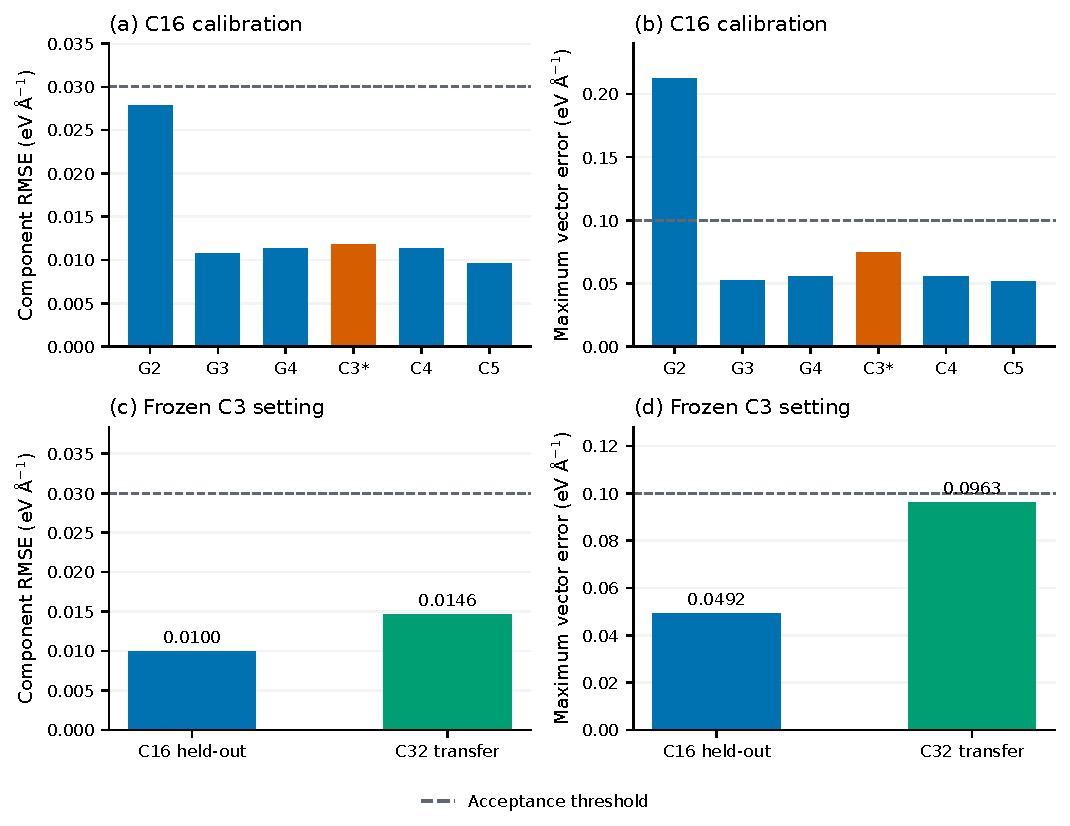
\includegraphics[width=\linewidth]{figures/fig03_fragment_fidelity.pdf}
  \caption{Fragment-fidelity calibration and transfer. G2--G4 denote
  graph neighborhoods of two to four bond hops; C3--C5 denote radial
  neighborhoods with a 1.5~\AA\ core and 3--5~\AA\ buffers. C3*, in
  orange, is selected by the recorded cost-and-tie rule. Upper panels
  show calibration; lower panels apply that setting to held-out C16
  and to two C32 parents. Dashed lines show the component-RMSE and
  maximum-vector-error acceptance thresholds. Bars are pooled
  deterministic evaluations of the available core atoms, not estimates
  with independent statistical error bars.}
  \label{fig:fidelity}
\end{figure}

\begin{table}[tb]
  \centering
  \small
  \caption{C16 calibration. Force errors are in \forceunit.
  Atom counts and allocated core-seconds are means over fragment
  specifications, including repeated structures.}
  \label{tab:calibration}
  \begin{tabular}{lrrrr}
\toprule
Setting & RMSE & Max.\ error & Mean atoms & Core-s/fragment \\
\midrule
Graph, 2 hops & 0.0278 & 0.2125 & 23.7 & 508 \\
Graph, 3 hops & 0.0108 & 0.0521 & 28.6 & 692 \\
Graph, 4 hops & 0.0113 & 0.0552 & 32.9 & 904 \\
Radial, 3 \AA\ buffer (selected) & 0.0118 & 0.0747 & 28.6 & 692 \\
Radial, 4 \AA\ buffer & 0.0113 & 0.0552 & 33.6 & 879 \\
Radial, 5 \AA\ buffer & 0.0095 & 0.0515 & 37.9 & 1095 \\
\bottomrule
\end{tabular}

\end{table}

Applied unchanged to seven sites from four held-out C16 parents, the
selected setting gives RMSE 0.0100~\forceunit\ and maximum error
0.0492~\forceunit. Four fragments from the two C32 parents give
0.0146 and 0.0963~\forceunit, respectively. Both pass, but the C32
maximum is close to the 0.10~\forceunit\ limit. Mean fragment size
increases from 28.6 to 33.3 atoms while the parent size increases from
50 to 98 atoms. This is a small transfer check across two chain lengths,
not a demonstration of asymptotic size independence.

Figure~\ref{fig:cost}(a) separates per-atom core errors by element and
distance to the cut. Carbon and hydrogen occupy different error ranges;
pooling them into a single component RMSE can hide the larger carbon
errors. The maximum-vector criterion supplies a complementary check.
The scatter does not by itself isolate a causal boundary effect from
element, conformation, or perturbation-site differences.

\begin{figure}[tb]
  \centering
  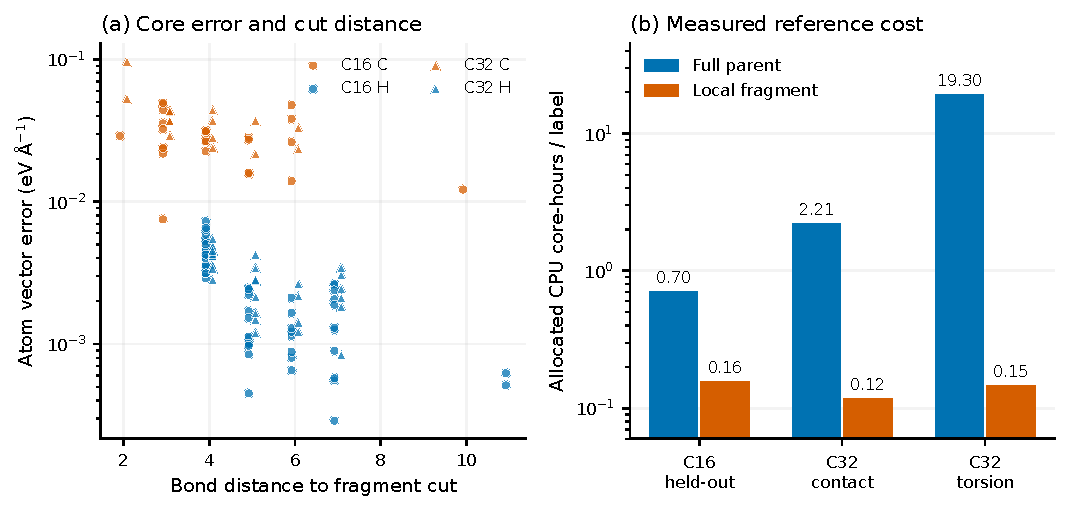
\includegraphics[width=\linewidth]{figures/fig04_boundary_and_cost.pdf}
  \caption{Core-force errors and reference cost for the selected
  fragment setting. (a) Each point is a retained core atom in one
  evaluated fragment; repeated atoms across sites remain separate.
  Horizontal offsets separate C16 circles from C32 triangles.
  Colors distinguish carbon and hydrogen. (b) Allocated cost includes
  all reference attempts. C16 bars are means over the seven held-out
  site specifications, so parents can enter repeatedly. Each C32 full
  bar is one parent calculation, and each local bar averages its two
  fragment calculations. Different box sizes and full-parent SCF
  retries contribute to the large C32 cost differences.}
  \label{fig:cost}
\end{figure}

The held-out C16 mean cost is 0.156~\coreh\ per fragment versus
0.704~\coreh\ for its corresponding full parent, using the
site-weighted means in Fig.~\ref{fig:cost}(b). On C32, the contact
parent costs 2.21~\coreh\ and its fragments average 0.117~\coreh;
the torsional parent costs 19.30~\coreh\ and its fragments average
0.146~\coreh. Both C32 parent jobs require an SCF retry, whereas
the four fragments do not. The parent box edges also differ, at
32.4 and 46.2~\AA. These measurements demonstrate a lower reference
cost for these particular fragments. They do not establish a general
speedup factor or a scaling law for CP2K.

\subsection{Exploratory acquisition comparison}
Figure~\ref{fig:acquisition} retains the individual trajectories of
both repetitions for all five arms. At four acquired labels,
PHAL local and PHAL full have mean held-out force RMSEs of
0.479 and 0.502~\forceunit\ (Table~\ref{tab:acquisition}). Their
mean attributed reference costs are 1948 and 10037 allocated
core-seconds, giving a local/full ratio of 0.194.
The four acquisitions coincide at the parent-and-site level in
the first repetition. They do not fully coincide in the second:
local selection acquires two sites of an ordinary parent, while
full-parent deduplication substitutes a bent parent for the second
ordinary-parent site. Thus the comparison is neither a strictly
paired test of fragment substitution nor a statistical equivalence test.

\begin{figure}[tb]
  \centering
  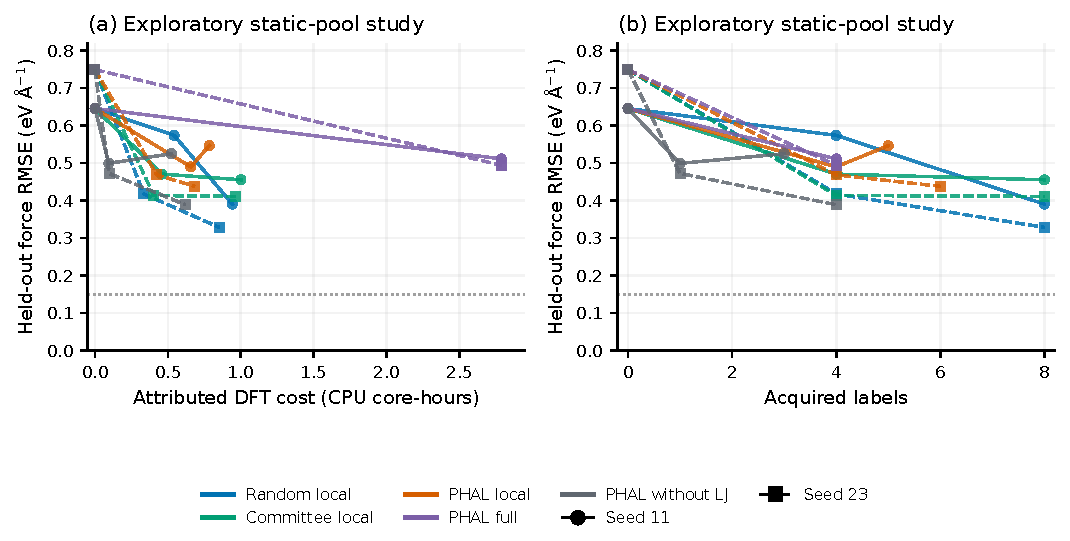
\includegraphics[width=\linewidth]{figures/fig05_acquisition.pdf}
  \caption{Completed exploratory static-pool acquisition study (v2c).
  Each marker is an evaluated model after an acquisition round;
  lines connect observations only and are not additional measurements.
  Solid circles and dashed squares identify the two seeds.
  The horizontal axes show attributed DFT cost and acquired label count.
  Costs charge cached labels at their historical measured reference cost;
  they exclude training, monitoring, and the shared initial dataset.
  The dotted line is the 0.15~\forceunit\ target, which no arm reaches.
  Parent deduplication stops the full-system arm after four labels.
  The final-evaluation set was inspected in earlier exploratory versions.}
  \label{fig:acquisition}
\end{figure}

\begin{table}[tb]
  \centering
  \small
  \caption{Directly observed four-label comparison. Force RMSEs are
  in \forceunit; costs are allocated core-seconds attributed to newly
  acquired labels. Arithmetic means summarize two repetitions without
  implying confidence intervals or equivalence.}
  \label{tab:acquisition}
  \begin{tabular}{lrrrr}
\toprule
Arm & \multicolumn{2}{c}{RMSE at four labels} & Mean RMSE & Mean core-s \\
& Seed 11 & Seed 23 & & \\
\midrule
Random local & 0.5736 & 0.4174 & 0.4955 & 1580 \\
Committee local & 0.4704 & 0.4132 & 0.4418 & 1554 \\
PHAL local & 0.4896 & 0.4683 & 0.4790 & 1948 \\
PHAL full & 0.5110 & 0.4937 & 0.5023 & 10037 \\
\bottomrule
\end{tabular}

\end{table}

Neither PHAL arm consistently outperforms the simpler acquisition
rules. At four labels the committee-ranked arm has mean RMSE
0.442~\forceunit, below the PHAL-local mean. After two rounds,
random acquisition reaches 0.390 and 0.328~\forceunit\ with eight
labels, whereas PHAL local reaches 0.546 and 0.438~\forceunit\ with
five and six labels. These final points have different acquisition
counts and costs. The first PHAL-local repetition worsens after its
second round. No arm reaches either recorded target, 0.15 or
0.10~\forceunit.

Removing the LJ residual reduces triggered structure--round evaluations
from eight of eight in each PHAL-local repetition to three of eight
and four of eight. These eight evaluations comprise four configurations
scored in each of two rounds. Its final errors, 0.525 and
0.389~\forceunit, do not
demonstrate an accuracy benefit from retaining that residual.
The feature affects acquisition behavior, but its incremental
predictive value is unresolved at this sample size.

\subsection{Real closed-loop execution and short-trajectory behavior}
The online pilot executes two GMD segments, collects ten events,
adds three CP2K fragment labels, and promotes two candidate models.
The first update occurs after 1~ps and supplies the second MD
segment. The second update occurs at 2~ps, after the online
trajectory has ended; it is evaluated in the separate frozen-model
trajectories. The fragments contain 44, 26, and 29 atoms and cost
1.054~\coreh\ in total. Validation force RMSE changes from
0.506 to 0.460 to 0.398~\forceunit, a 21.4\% reduction from the
initial value (Fig.~\ref{fig:closed}).

\begin{figure}[tb]
  \centering
  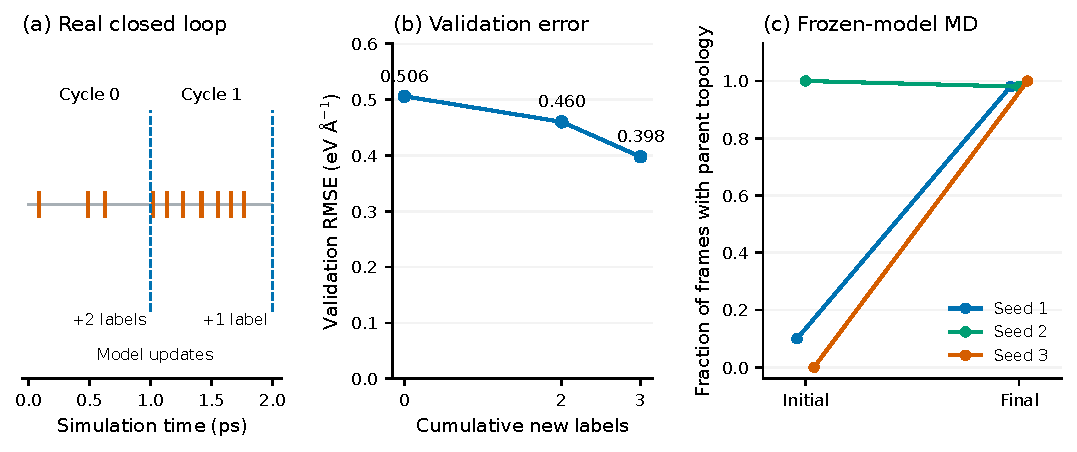
\includegraphics[width=\linewidth]{figures/fig06_closed_loop.pdf}
  \caption{Real-program closed-loop pilot. (a) Orange ticks mark
  recorded events; blue dashed lines mark cycle boundaries at which
  two and then one local labels are incorporated. (b) Validation
  force RMSE after the initial model and the two promotions.
  (c) Fraction of sampled frames retaining the original bond topology
  for each of three velocity seeds under the frozen initial and final
  models. Each point summarizes 151 correlated frames from one short
  trajectory; the points are not independent-frame survival estimates.
  The final model is produced at the end of panel (a) and is tested
  separately in panel (c).}
  \label{fig:closed}
\end{figure}

In the frozen-model evaluation, the initial model retains the
parent topology in 15, 151, and 0 of 151 analyzed frames for the
three seeds. The final model retains it in 148, 148, and 151 frames.
The pooled descriptive fractions are therefore 36.6\% and 98.7\%.
This is an improvement in short-trajectory topology retention, with
brief departures still present under the final model. Frame
autocorrelation and only three trajectories preclude treating the
453 frames as independent replicates. Because the initial model
already fails on an ordinary starting structure, the example does
not establish repair of a qualified model outside its training domain.

Triggering is frequent even on the ordinary initial trajectory.
All ten recorded events include force, committee, and LJ reasons.
In the second cycle, the diversity filter rejects six of seven
candidates and the remaining candidate is labeled. The label budget
and duplicate filter therefore have a substantial role in controlling
reference cost. These records demonstrate working event-to-label
selection, but not a low false-alarm rate.

\subsection{Recovery and rollback}
Separate local fault-injection runs exercise the persistent controller
against real external programs. After termination of the controller
while CP2K remains alive, restart adopts the existing task, collects
its label once, trains and promotes a candidate, and resumes MD.
No extra task directory or duplicate reference attempt is created
in this case. A subsequent deliberately strict validation-gate audit
rejects the promoted model and restores the original accepted model
before MD resumes.
A CP2K cancellation probe passes its eight recorded checks, including
termination and absence of automatic resubmission. These are concrete
integration checks on the local five-thread backend, not evidence
for every scheduler or multi-node failure scenario.

\section{Discussion and limitations}
The strongest scientific result in this pilot is the measured fidelity
of selected local DFT labels. The cost reduction is useful only because
the retained core forces are compared directly with full-parent
references. The failed two-hop setting illustrates why a pooled average
alone is insufficient. The C32 transfer further shows that a setting
chosen on a smaller molecule can remain useful on a larger parent,
although its near-threshold maximum error calls for caution.

The strongest systems result is that those labels can pass through
the complete dynamics--monitoring--reference--training cycle with
recorded provenance, weighted supervision, promotion, and recovery.
This integration complements prior local active-learning methods;
it does not establish priority for local selection or closed-loop
learning. The platform's physics-aware features are candidate
diagnostics. Their value must be measured against reference-force
errors and simpler acquisition rules, rather than inferred from
their physical motivation.

Several observations limit that interpretation here. The static
comparison contains only two repetitions and a small, repeatedly
examined final-evaluation set. Its PHAL thresholds trigger every
available static frame, and the no-LJ comparison does not reveal
a consistent advantage from the LJ feature. An earlier reference-error
audit labels all 64 evaluated regions positive at each of the
0.1, 0.2, and 0.4~\forceunit\ thresholds. The audit accordingly
does not report average precision as an informative discrimination
metric. With no negative regions, the experiment cannot assess
specificity in distinguishing acceptable from erroneous environments.
Event buffering also has no demonstrated benefit from the static-pool
comparison, which scores unrelated configurations independently.

There is a further distinction between electronic locality and model
locality. A completed diagnostic on one central carbon of one C16
structure finds trained-model force sensitivity extending to roughly
7.6~\AA; truncation to 3~\AA\ can alter that force, whereas
truncation at 8~\AA\ falls below the diagnostic's
$10^{-4}$~\forceunit\ tolerance. The random model has a much smaller
effective range in the same probe. These observations show that a
single-layer cutoff or an untrained-model probe does not determine
the context needed by a trained force prediction. The selected
fragment's DFT-fidelity pass therefore does not eliminate a possible
parent--fragment representation mismatch. This diagnostic is limited
to one model, structure, atom, and perturbation procedure.

The closed-loop topology improvement is encouraging but its initial
model is not a sound baseline for claiming extrapolation repair.
Nor can 2~ps trajectories establish equilibrium conformational
statistics, rare-event kinetics, or long-time stability. An energy
jump of 2.246~eV occurs at a fixed-coordinate model replacement;
this is a change of potential-energy function, not integrator drift.
Energy conservation across model switches is therefore not claimed.
The periodic-box checks support the short trajectories actually
run, not arbitrary later molecular extension.

The evidence supports a platform and an exploratory local-label study.
A stronger repair claim requires an initially qualified force field,
independent confirmation of out-of-domain failures, paired controls
for extra training and acquisition, and a separate final assessment
of both repair and retention of in-domain accuracy. No outcomes
from such an unfinished experiment are included here.


\section{Conclusions}
PHAL integrates local reference labeling with a persistent active-learning
workflow in the GMD ecosystem. Completed alkane experiments show that
hydrogen-capped fragments of approximately thirty atoms can reproduce parent
core forces within explicitly checked tolerances, including a small
transfer from C16 to C32. Real dynamics, reference calculations, training,
model replacement, interruption recovery, and rollback have been exercised
in the same implementation. The short closed-loop example also shows
improved validation error and topology retention after three local labels.
The evidence remains exploratory: it does not establish superior acquisition,
equilibrium accuracy, or reliable extrapolation repair.
The contribution is a documented integration and validation of the local-label
workflow, together with explicit tests of where its present evidence stops.

\section*{Code and data availability}
The accompanying manuscript source package contains frozen result summaries,
per-atom fragment-error tables, acquisition records, molecular coordinates
used in the illustrations, configuration snapshots, and scripts that regenerate
all figures and numerical tables. A provenance manifest records the source
paths and SHA-256 hashes. Figure regeneration uses only these bundled data.
The package does not include the complete CP2K output archive, all dynamics
trajectories, or trained model checkpoints. No public repository or archival
identifier is asserted in this draft.

\section*{Use of generative AI tools}
Generative AI tools assisted manuscript drafting, source inspection,
reference checking, and preparation of plotting and validation scripts.
The reported numerical measurements come from recorded simulation and
training artifacts; no generative model supplied simulation measurements.

\section*{Acknowledgments}
\PaperAcknowledgments

\section*{Author contributions}
[CRediT contributions to be supplied and approved by the authors.]

\section*{Competing interests}
[Competing-interest declaration to be supplied by the authors.]

\section*{Ethics declaration}
The reported work concerns computational molecular systems and does not
involve human participants, personal data, or animal experiments.

\FloatBarrier
% Explicit bibliography supplied so the source does not depend on a generated .bbl.
% Editable BibTeX metadata are also supplied in references.bib.
\begin{thebibliography}{11}
\bibitem{podryabinkin2017active}
E. V. Podryabinkin and A. V. Shapeev,
Active learning of linearly parametrized interatomic potentials,
\emph{Computational Materials Science} \textbf{140}, 171--180 (2017).
\href{https://doi.org/10.1016/j.commatsci.2017.08.031}{doi:10.1016/j.commatsci.2017.08.031}.

\bibitem{vandermause2020flare}
J. Vandermause, S. B. Torrisi, S. Batzner, Y. Xie, L. Sun,
A. M. Kolpak, and B. Kozinsky,
On-the-fly active learning of interpretable Bayesian force fields for
atomistic rare events,
\emph{npj Computational Materials} \textbf{6}, 20 (2020).
\href{https://doi.org/10.1038/s41524-020-0283-z}{doi:10.1038/s41524-020-0283-z}.

\bibitem{zhang2020dpgen}
Y. Zhang, H. Wang, W. Chen, J. Zeng, L. Zhang, H. Wang, and W. E,
DP-GEN: A concurrent learning platform for the generation of reliable
deep learning based potential energy models,
\emph{Computer Physics Communications} \textbf{253}, 107206 (2020).
\href{https://doi.org/10.1016/j.cpc.2020.107206}{doi:10.1016/j.cpc.2020.107206}.

\bibitem{hodapp2020inoperando}
M. Hodapp and A. Shapeev,
In operando active learning of interatomic interaction during large-scale
simulations,
\emph{Machine Learning: Science and Technology} \textbf{1}, 045005 (2020).
\href{https://doi.org/10.1088/2632-2153/aba373}{doi:10.1088/2632-2153/aba373}.

\bibitem{podryabinkin2023mlip3}
E. Podryabinkin, K. Garifullin, A. Shapeev, and I. Novikov,
MLIP-3: Active learning on atomic environments with moment tensor potentials,
\emph{The Journal of Chemical Physics} \textbf{159}, 084112 (2023).
\href{https://doi.org/10.1063/5.0155887}{doi:10.1063/5.0155887}.

\bibitem{larsen2017ase}
A. H. Larsen \emph{et al.},
The atomic simulation environment---a Python library for working with atoms,
\emph{Journal of Physics: Condensed Matter} \textbf{29}, 273002 (2017).
\href{https://doi.org/10.1088/1361-648X/aa680e}{doi:10.1088/1361-648X/aa680e}.

\bibitem{kuhne2020cp2k}
T. D. K\"uhne \emph{et al.},
CP2K: An electronic structure and molecular dynamics software package---Quickstep:
Efficient and accurate electronic structure calculations,
\emph{The Journal of Chemical Physics} \textbf{152}, 194103 (2020).
\href{https://doi.org/10.1063/5.0007045}{doi:10.1063/5.0007045}.

\bibitem{perdew1996pbe}
J. P. Perdew, K. Burke, and M. Ernzerhof,
Generalized gradient approximation made simple,
\emph{Physical Review Letters} \textbf{77}, 3865--3868 (1996).
\href{https://doi.org/10.1103/PhysRevLett.77.3865}{doi:10.1103/PhysRevLett.77.3865}.

\bibitem{grimme2010d3}
S. Grimme, J. Antony, S. Ehrlich, and H. Krieg,
A consistent and accurate ab initio parametrization of density functional
dispersion correction (DFT-D) for the 94 elements H--Pu,
\emph{The Journal of Chemical Physics} \textbf{132}, 154104 (2010).
\href{https://doi.org/10.1063/1.3382344}{doi:10.1063/1.3382344}.

\bibitem{grimme2011d3bj}
S. Grimme, S. Ehrlich, and L. Goerigk,
Effect of the damping function in dispersion corrected density functional theory,
\emph{Journal of Computational Chemistry} \textbf{32}, 1456--1465 (2011).
\href{https://doi.org/10.1002/jcc.21759}{doi:10.1002/jcc.21759}.

\bibitem{vandevondele2007molopt}
J. VandeVondele and J. Hutter,
Gaussian basis sets for accurate calculations on molecular systems in gas
and condensed phases,
\emph{The Journal of Chemical Physics} \textbf{127}, 114105 (2007).
\href{https://doi.org/10.1063/1.2770708}{doi:10.1063/1.2770708}.
\end{thebibliography}

\appendix
\section{Additional implementation and evaluation details}
\label{app:settings}
\subsection{Monitoring and geometry}
The LJ fit uses column-normalized least squares on a $3\times2$
matrix. It requires rank two, a normalized condition number no greater
than $10^4$, positive fitted coefficients, and a fitted
$\sigma=(\alpha/\beta)^{1/6}$ between 0.2 and 10~\AA.
The residual denominator uses $\delta=10^{-8}$ in the force units
of Eq.~\eqref{eq:lj}; invalid fits receive residual one.
The check concerns compatibility of one force vector with a local
pair-force basis. It does not test energy conservation, a full force
Jacobian, or a transferable LJ parameterization across atoms.

The diversity fingerprint comprises 16-bin geometric summaries of
pair-distance density, atomic-number-weighted density, and weighted
bin means, giving 48 components with an 8~\AA\ cutoff.
The selector compares fingerprint distances against the configured
0.1 threshold. In a pending event, later triggers merge hotspot and
reason records without repeatedly extending the original post-event
window. Both completed and truncated events preserve completeness
information. These details describe the implementation; the pilot
does not separately estimate each design choice's causal contribution.

\subsection{Training and evaluation conventions}
The static study uses a minimum learning rate of $2\times10^{-5}$,
50 warm-up optimizer steps, one attention head, maximum angular momentum one,
and an average-neighbor setting of 12. Closed-loop fine-tuning uses
five warm-up optimizer steps. The bundled configuration snapshots contain
the remaining recorded settings and their inheritance references.
They are provenance records, not standalone configurations for
launching new calculations from this manuscript directory.

Reported model force errors pool Cartesian components across the
evaluated atoms. Fragment maximum errors instead use the Euclidean
norm of each atom's three-component error. Local-label force weights
apply during training, not as a way to hide atoms in the full-parent
evaluation metric. The atomwise fidelity data retain repeated
atom--fragment observations, since a parent atom can appear in
more than one independently extracted site.

For the closed-loop trajectory, all 401 saved frames have nearest-image
separation above 20.7~\AA. Across the initial/final frozen-model runs,
the 1206 checked frames have minimum separation approximately
18.76~\AA. None violates the nominal 16~\AA\ force-dependence bound,
although 82 frames fall within a further 4~\AA\ caution margin.
These checks assess the recorded finite trajectories only.

\subsection{Exploratory protocol history}
Earlier static-pool configurations did not exercise the intended
PHAL acquisition path. The archived v2 run records zero PHAL-local
and PHAL-full acquisitions because the light-stage trigger does not
activate the higher stages. Its zero-acquisition ablations therefore
do not measure the benefit of local learning. The executed v2c
comparison follows corrections to static-frame event handling and
candidate mapping and explicitly evaluates every stage. We report
that configuration as an exploratory comparison, not as a
prospectively fixed experiment. Figures contain directly evaluated
rounds; interpolated budget metrics in the archived reports are not
presented as observations.

\section{Artifact contents and reproduction}
The source package supplies six figures in vector PDF and SVG formats
and PNG previews. Their inputs are frozen in
\texttt{data/plot\_data.json}; source records, configuration snapshots,
and hashes accompany them. The plotting script regenerates the figures
and two numerical tables without invoking GMD, CP2K, or GMD\_SGT.
A separate bundle validator checks file references, citation keys,
snapshot hashes, and numerical consistency against the per-atom
and per-run records. These checks do not replace author review of
the scientific interpretation or a final typesetting inspection.

\end{document}
